%! TEX root = FisicaII.tex

\documentclass{./FisicaII.tex}

\begin{document}
\chapter{Potencial Eléctrico}
\section{Trabajo y energía potencial}
Supongamos una carga $q_{2}$, sometida a un determinado campo eléctrico $\mathbf{E}$, generado por una carga $q_{1}$ (en reposo). La carga $q_{2}$ se sitúa inicialmente  en $\mathbf{r}_{i}$, y se desplaza, bajo el efecto del campo eléctrico, hasta $\mathbf{r}_{f}$.\\
Este trabajo, aplicando la ley de Coulomb, termina siendo
$$
W=\int_{r_{i}}^{r_{f}} \frac{1}{4\pi\varepsilon_{0}} \frac{q_{1}q_{2}}{r^2}dr = -\left( \frac{q_{1}q_{2}}{4\pi\varepsilon_{0}r_{f}} - \frac{q_{1}q_{2}}{4\pi\varepsilon_{0}r_{i}} \right)=U_{i}-U_{f}=-\Delta U
$$
de aquí se deduce que el trabajo depende de la función **energía potencial** $U$. Esta depende únicamente de la posición de la partícula $q_{2}$ en cada momento $t$, y viene dada por

$$
\boxed{
U=\frac{1}{4\pi\varepsilon_{0}} \frac{q_{1}q_{2}}{|r|}
}
$$
El trabajo realizado al desplazar la carga de $\mathbf{r}_{i}$ a $\mathbf{r}_{f}$ se puede expresar como la diferencia de la energía potencial:
$$
W=-\Delta U
$$
De aquí se puede deducir que el trabajo realizado para desplazar no depende de la trayectoria, sino únicamente de lo punto inicial y final.
\section{Potencial eléctrico}
Si la carga receptora $q_{2}$ está sometida a un campo eléctrico $\mathbf{E}$, se cumple que la fuerza generada es $\mathbf{F}=q_{2}\mathbf{E}$. Por tanto, el trabajo realizado por el campo eléctrico al desplazar $q_{2}$ se puede definir como
\begin{equation}
	\begin{split}
W&=\int_{r_{i}}^{r_{f}}q_{2}\mathbf{E}\cdot \mathbf{dr}\\
\frac{W}{q_{2}} &= \int_{r_{i}}^{r_{f}}\mathbf{E}\cdot \mathbf{dr}\\
\frac{W}{q_{2}}&= \frac{q_{1}}{4\pi\varepsilon_{0}r_{i}}-\frac{q_{1}}{4\pi\varepsilon_{0}r_{f}}=-\Delta V
	\end{split}
\end{equation}
por tanto, definimos el potencial eléctrico como
$$
\boxed{
V(r) = \frac{q_{1}}{4\pi\varepsilon_{0}r}~ \left( \frac{J}{C} \right) = \frac{U}{q_{2}}~(V)
}
$$
que es la energía potencial por unidad de carga. También podemos deducir que
$$
[E]=\left[ \frac{V}{m} \right]
$$
Si sabemos la expresión de un campo elécitro, se da que
\begin{equation}
	\begin{split}
		V(\vb{r}) - V(\infty) = -\int_{\infty}^{\vb{r}}\vb{E}\cdot \dd{\vb{r}}
	\end{split}
\end{equation}
\section{Campo vectorial}
Supongamos una carga $q_{1}$ que genera un campo eléctrico $\mathbf{E}$ sobre una carga de $1~(C)$ a una distancia $r$ del foco. Se dice que $\mathbf{E}$ es conservativo si cumple que:\\
- $\mathbf{E}$ solo depende de la posición, y no depende explícitamente del tiempo.\\
- Si se cumple $1$, existe una función $V(\mathbf{r})$ tal que $V(\mathbf{r}_{i})\\
- V(\mathbf{r}_{f})=\frac{W}{q_{2}}$. La diferencia de potencial solo depende de la posición inicial y final de la carga desplazada.\\
- La integral del trabajo a lo largo de un camino cerrado es $0$. Consecuentemente, la circulación de un vector siempre es nula.\\
- $dV=-\mathbf{E}\cdot \mathbf{dr}$
\section{Potencial por una distribución de carga}
Supongamos un conjunto de cargas que se denotan $\{ q_{i} \}^{n}$, la posición relativa de cada carga al punto $P$ se denota $\mathbf{r}_{i}$.\\
El potencial en $P$ es la suma de potenciales inviduales:
\begin{equation}
	\begin{split}
		V(\mathbf{r}_{P}) = \sum_{i=1}^{n} \frac{1}{4\pi \varepsilon_{0}}
		\frac{q_{i}}{|\mathbf{r}_{i}|}
	\end{split}
\end{equation}
\section{Potencial por distribución de carga continua}
\subsection{Lineal}
El potencial debido a una distribución de carga lineal con densidad de carga
\[
	\lambda = \dv{q}{l}
\]
Al tener una carga infinitesimal $\dd{q}$, le corresponde un potencial infinitesimal $\dd{V}$, por lo que, integrando, tenemos
\begin{equation}
	\begin{split}
		V(r) = \int \frac{1}{4\pi \varepsilon_{0}} \frac{\lambda \dd{l}}{|r|}
	\end{split}
\end{equation}
\subsection{Superficie equipotencial}
Una superfície equipotencial (Figura \ref{fig:superficie-equipotencial}) es el conjunto de puntos donde el potencial en cada uno de ellos es el mismo. En una superfície equipotencial, se cumple que $V(\vb{r})=C$, por lo que
\[
	\pdv{V}{r}=0
\]
Las líneas de campo siempre son perpendiculares a la superfície equipotencial.
\begin{figure}[ht]
    \centering
    \incfig{superficie-equipotencial}
    \caption{Superfície Equipotencial}
    \label{fig:superficie-equipotencial}
\end{figure}
\pagebreak
\section{Principios de la transferencia de la carga en un conductor}
\begin{itemize}
	\item Si el potencial asociado a una superfície equipotencial es distinto de $0$, entonces la carga neta del cuerpo es no nula.
	\item Las superfícies equipotenciales no se cortan entre sí.
	\item El campo eléctrico en una esfera conductora asociada a una superfície equipotencial (con potencial no nulo) siempre es perpendicular a la superfície.
\end{itemize}
\begin{figure}[ht]
\centering


\tikzset{every picture/.style={line width=0.75pt}} %set default line width to 0.75pt

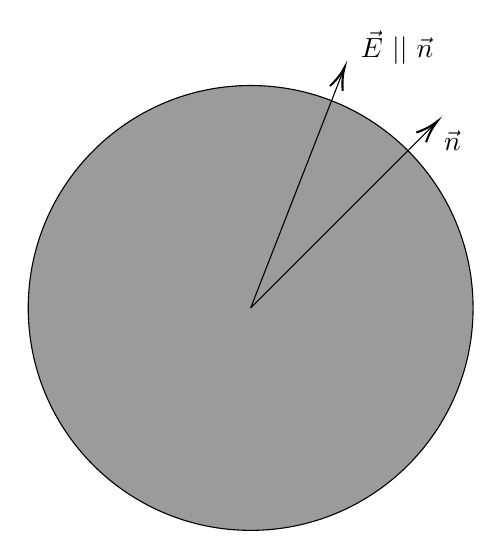
\begin{tikzpicture}[x=0.75pt,y=0.75pt,yscale=-1,xscale=1]
%uncomment if require: \path (0,300); %set diagram left start at 0, and has height of 300

%Shape: Circle [id:dp34897156253908657]
\draw  [fill={rgb, 255:red, 155; green, 155; blue, 155 }  ,fill opacity=1 ] (181,158.17) .. controls (181,98.98) and (228.98,51) .. (288.17,51) .. controls (347.35,51) and (395.33,98.98) .. (395.33,158.17) .. controls (395.33,217.35) and (347.35,265.33) .. (288.17,265.33) .. controls (228.98,265.33) and (181,217.35) .. (181,158.17) -- cycle ;
%Straight Lines [id:da061641948648095135]
\draw    (288.17,158.17) -- (376.67,69.66) ;
\draw [shift={(378.08,68.25)}, rotate = 135] [color={rgb, 255:red, 0; green, 0; blue, 0 }  ][line width=0.75]    (10.93,-3.29) .. controls (6.95,-1.4) and (3.31,-0.3) .. (0,0) .. controls (3.31,0.3) and (6.95,1.4) .. (10.93,3.29)   ;
%Straight Lines [id:da12243663771403401]
\draw    (288.17,158.17) -- (332.69,44.11) ;
\draw [shift={(333.42,42.25)}, rotate = 111.32] [color={rgb, 255:red, 0; green, 0; blue, 0 }  ][line width=0.75]    (10.93,-3.29) .. controls (6.95,-1.4) and (3.31,-0.3) .. (0,0) .. controls (3.31,0.3) and (6.95,1.4) .. (10.93,3.29)   ;

% Text Node
\draw (340,23.4) node [anchor=north west][inner sep=0.75pt]    {$\vec{E} \ ||\ \vec{n}$};
% Text Node
\draw (380.08,71.65) node [anchor=north west][inner sep=0.75pt]    {$\vec{n}$};


\end{tikzpicture}
\caption{Campo perpendicular a la superfície}
\label{fig:campo-perp-super}
\end{figure}
Se da siempre que
\[
	W =	\int_{B}^{A} \vb{E}\cdot \dd{\vb{r}} = 0
\]
Esto es debido a que el potencial es constante, además de que el campo $\vb{E}$ es perpendicular a la dirección de desplazamiento. Si la carga es distinta de $0$ , el campo no puede ser nulo. Por tanto, tenemos dos opciones:
\begin{itemize}
	\item El campo es perpendicular: $\vb{E} \perp \vb{n}$
	\item En el interior del conductor, el campo eléctrico $\vb{E}$ es nulo, por tanto, también se cumple que $\int_{B}^{A} \vb{E}\cdot \dd{\vb{r}}=0$, debido a que la carga en el interior es $0$. 
\end{itemize}
Esto se cumple tanto en las superfícies equipotenciales de exterior como las superficies equipotenciales del interior del conductor que este está en equilibrio eléctrico: las cargas están en reposo.
\[
	\Delta V = 0 \implies \Delta T = 0
\]
\section{Transferencia de carga}
 Si el campo eléctrico es conservativo, el sistema se va a comportar de forma que llegue a su estado de menor energía potencial. Si se traslada una unidad carga positiva, se pasa de un potencial mayor a uno menor, y el sistema llega al equilibrio cuando el potencial se mantiene constante.
\section{Movimiento de cargas entre conductores}
Supongamos dos conductores esféricos en equilibrio electroestático (cargas inmóviles). Los conductores tenderán a su estado de menor energía potencial.\\
La primera esfera tiene un radio $r_1$ y una carga en la superfície $q_1$.
\[
	V_1 = \frac{1}{4\pi \varepsilon_0} \frac{q_1}{r_1}
\]
La segunda esfera tiene un radio y carga $r_2$ y $q_2$, respectivamente, con un potencial  
\[
	V_2 = \frac{1}{4\pi \varepsilon_0} \frac{q_2}{r_2}
\]
Definamos un nuevo parámetro llamado 'capacidad del conductor'. Esta es la relación entre la carga y su potencial:
\[
	C = \frac{q}{V} \implies [C] = 1 faradio = \frac{C}{V}
\]
Por tanto, la capacidad del primer conductor es
\[
	C_1 = \frac{q_1}{V_1} = 4\pi \varepsilon_0 r_1 = \frac{r}{k}
\]
Si unimos ambas esferas por un hilo metálico o conductor, tiene lugar la transferencia de carga de una esfera con mayor potencial a otra con menor potencial. Cuando se llega al equilibrio electroestático, el potencial de ambas esferas coincide.
\begin{figure}[ht]
\centering


\tikzset{every picture/.style={line width=0.75pt}} %set default line width to 0.75pt

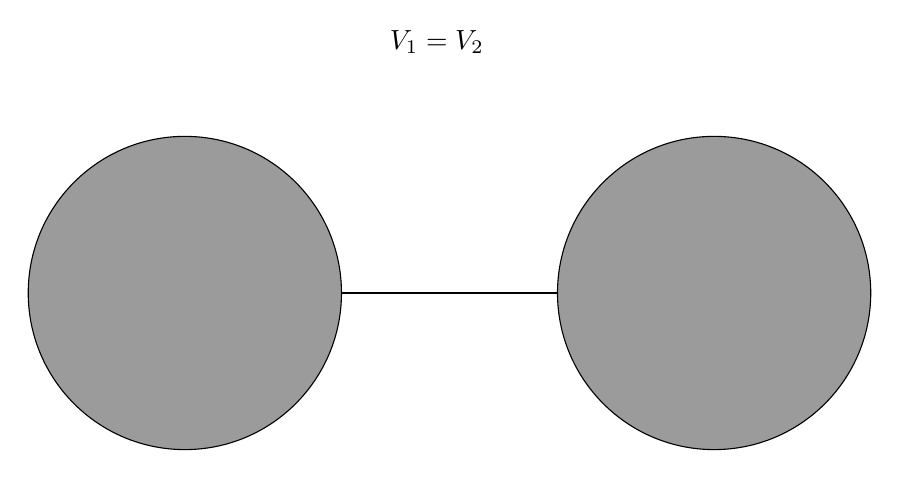
\begin{tikzpicture}[x=0.75pt,y=0.75pt,yscale=-1,xscale=1]
%uncomment if require: \path (0,300); %set diagram left start at 0, and has height of 300

%Shape: Circle [id:dp017061440553987173]
\draw  [fill={rgb, 255:red, 155; green, 155; blue, 155 }  ,fill opacity=1 ] (113.08,178.96) .. controls (113.08,137.28) and (146.87,103.5) .. (188.54,103.5) .. controls (230.22,103.5) and (264,137.28) .. (264,178.96) .. controls (264,220.63) and (230.22,254.42) .. (188.54,254.42) .. controls (146.87,254.42) and (113.08,220.63) .. (113.08,178.96) -- cycle ;
%Shape: Circle [id:dp7170792528720665]
\draw  [fill={rgb, 255:red, 155; green, 155; blue, 155 }  ,fill opacity=1 ] (368.08,178.96) .. controls (368.08,137.28) and (401.87,103.5) .. (443.54,103.5) .. controls (485.22,103.5) and (519,137.28) .. (519,178.96) .. controls (519,220.63) and (485.22,254.42) .. (443.54,254.42) .. controls (401.87,254.42) and (368.08,220.63) .. (368.08,178.96) -- cycle ;
%Straight Lines [id:da39442064776804153]
\draw    (264,178.96) -- (368.08,178.96) ;

% Text Node
\draw (286,51.4) node [anchor=north west][inner sep=0.75pt]    {$V_{1} =V_{2}$};


\end{tikzpicture}

\end{figure}
\\
\textbf{Ejemplo}: sean 2 esferas conductoras aisladas, dadas las siguientes condiciones:
\begin{itemize}
	\item Esfera 1: $r_1 = 2~cm, q_1 = 1~nC$ 
	\item Esfera 2: $r_2 = 4~cm, q_2=3~nC$ 
\end{itemize}
Determina el potencial de cada esfera y las capacidades de ambas esferas.
\[
	V_1 = k \frac{q_1}{r_1} = 450~(V)
\]
\[
	V_2 = k \frac{q_2}{r_2} = 675~(V)
\]
Si se unen ambas esferas por un hilo conductor, ¿cuál seria la carga transferida de una esfera a otra?\\
La carga irá de la segunda esfera a la primera, por lo que planteamos las siguientes ecuaciones:
\begin{equation}
	\begin{split}
		V_1 &= V_2\\
		q_1+q_2 &= q_1'+q_2'
	\end{split}
\end{equation}
Con esto obtenemos que
\begin{equation}
	\begin{split}
		q_1' &= 1.34~(nC)\\
		q_2' &= 2.66~(nC)
	\end{split}
\end{equation}
\section{Energía electroestática asociada a cargas puntuales}
Supongamos dos cargas puntuales, con la distancia relativa entre ellas siendo $r_{1,2}$. Se puede expresar el trabajo realizado para transportar la carga $q_1$ desde el infinito hasta $r_{1,2}$ debido al campo eléctrico generado por $q_2$. La energía electroestática es:
\begin{equation}
	\begin{split}
		U = \frac{1}{4\pi\varepsilon_0} \frac{q_1q_2}{r_{1,2}}~(J)
	\end{split}
\end{equation}
Sin embargo, esto genera problemas cuando la cantidad de cargas aumenta. Podemos expresar el potencial anterior como
\begin{equation}
	\begin{split}
		U = \frac{1}{2}q_1 k \frac{q_2}{r} + \frac{1}{2} q_2 k \frac{q_2}{r}
	\end{split}
\end{equation}
Podemos generalizar esto a un número $n$ de cargas:
\begin{equation}
	\begin{split}
		U = \frac{1}{2} \sum_{i=1}^{n}q_{i} \sum_{j=1,i\neq j}^{n}k \frac{q_{j}}{r_{i,j}}~(J)
	\end{split}
\end{equation}
Que sería el equivalente al potencial de todo el sistema.
\end{document}
